%% ESWA (Expert Systems with Applications) 双栏投稿模板
%% 官方 elsarticle 文档类，5p = 双栏期刊版式（ESWA 终版格式）
%% 本地无 TeX 环境时，请在 Windows 侧 TeX Live 2025 或 Overleaf 编译
\documentclass[final,5p,times,twocolumn]{elsarticle}

\usepackage{amsmath,amssymb}
\usepackage{booktabs}
\usepackage{multirow}
\usepackage{graphicx}
\usepackage{algorithm}
\usepackage{algpseudocode}
\usepackage{xcolor}
\usepackage{url}

\journal{Expert Systems with Applications}

\begin{document}

\begin{frontmatter}

\title{Selective Cross-Model Verification for Emotion Recognition
in Conversations: When and Why Heterogeneous Review Helps}

%% 双盲投稿版本：作者与单位匿名（终稿恢复作者信息）
\author[1]{Anonymous Author\corref{cor1}}
\ead{anon@example.com}
\cortext[cor1]{Corresponding author}
\affiliation[1]{organization={Anonymous Institution}, city={City}, country={Country}}

\begin{abstract}
%% 初步填充：基于 8-seed 主结果与效率叙事
Emotion recognition in conversation (ERC) with fine-tuned large language
models (LLMs) has reached strong accuracy, yet errors concentrate on a
hard-to-detect minority of utterances. We introduce \emph{gated
heterogeneous review}, a deployment-time wrapper that augments an
\emph{already trained} ERC classifier without retraining it: a second,
heterogeneous LLM serves as a selective verifier that is invoked
only when the primary model is uncertain. On MELD (7-class) with eight
independent seeds, gated heterogeneous review improves weighted-F1 by
$+0.49 \pm 0.46$ percentage points (paired $t$: $p=0.019$; bootstrap 95\%
CI $[+0.18, +0.77]$; Cohen's $d_z=1.07$) at an expected cost of only
$1.27\times$ forward passes ($1.33\times$ in measured batch-1 wall-clock
latency, 2.38 utterances/s on a single 48\,GB GPU), while cheaper
alternatives all fail:
self-consistency
sampling (three paired seeds, two temperatures; 11 of 12 configurations
negative, $-0.08$ to $-1.45$), homogeneous self-debate
($-0.64$), and a weak 1.5B verifier ($-0.05$). A same-lineage Mistral-7B reviewer matched in standalone
accuracy and routing rate, by contrast, yields no significant gain
($+0.18 \pm 0.52$, eight seeds, paired $p{=}0.37$), localising the effect
to family-level independence rather than reviewer capability. The gain
transfers to IEMOCAP ($+1.21 \pm 0.42$,
three seeds, paired $p{=}0.037$) with adapters retrained on IEMOCAP and
only the gate hyperparameters frozen from MELD.
An eight-seed role reversal (Qwen2.5 proposes, LLaMA2 reviews) independently
replicates the gain ($+0.71 \pm 0.42$, 8/8 seeds, paired $p{=}0.002$), with
no significant difference between the two pairing directions.
Stacking the gate on an independently trained InstructERC primary further
shows the \emph{mechanism} is portable across training pipelines, while its
thresholds are not: generation-style confidence requires dev-level
recalibration (two-threshold variant, $+1.33$). A frozen cross-register
transfer to spontaneous DailyDialog chat
does not replicate the gain, bounding the transfer claim to matched
registers. Controlled analysis shows the benefit
is multiplicative in verifier independence and capability, and concentrates
in the high-coverage regime where abstention is disallowed.
\end{abstract}

\begin{keyword}
Emotion recognition in conversation \sep Large language models \sep
Selective prediction \sep Model verification \sep Cost-aware inference
\end{keyword}

\end{frontmatter}

\section{Introduction}
\label{sec:intro}
%% 动机段——ERC 错误集中于低置信少数样本（Fig.1 应用场景图，非架构图）
Emotion recognition in conversation (ERC) is increasingly considered for
high-volume applications such as contact-center quality inspection and
affective monitoring (we treat these as illustrative deployment settings; our
training corpora are scripted and acted transcripts, see
Section~\ref{sec:limitations}), where errors on a small fraction of
utterances, namely short, sarcastic, or context-dependent
turns, carry disproportionate cost. Figure~\ref{fig:scenario} illustrates the
operating point we target: a fine-tuned LLM labels each utterance online, and
its own label-sequence posterior already identifies where errors concentrate
(accuracy rises monotonically from 0.48 in the lowest confidence bucket to
0.90 in the highest). The question is how to exploit this signal.

\begin{figure}[t]
\centering
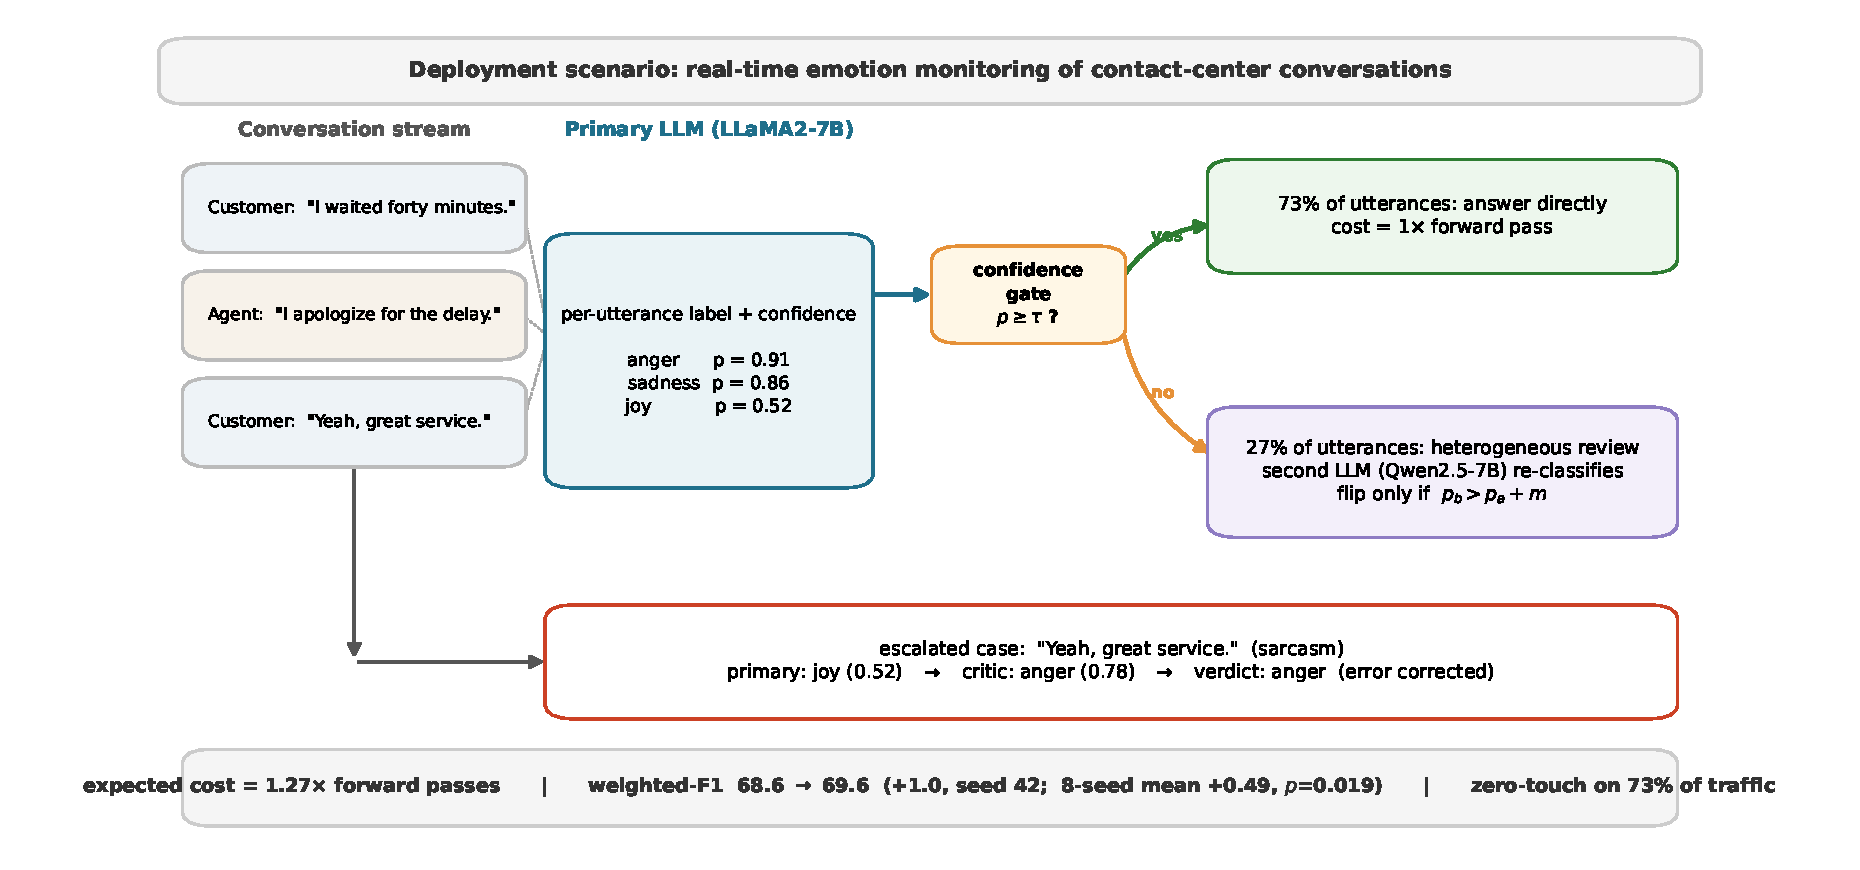
\includegraphics[width=\linewidth]{figures/fig_scenario.pdf}
\caption{Application scenario. A primary LLM labels the conversation stream
with calibrated confidences; only the low-confidence tail (27\% of traffic)
is escalated to a heterogeneous reviewer, correcting errors such as sarcastic
anger misread as joy at an expected cost of $1.27\times$ forward passes.}
\label{fig:scenario}
\end{figure}

Our first finding is negative and constrains the design space: spending more
compute on the \emph{same} model does not help. Homogeneous self-debate
reduces weighted-F1 by 0.64 points: two copies of one model agree on
91.3\% of utterances, including their mistakes, and self-consistency
sampling at 3--5$\times$ budget degrades accuracy by 1.5--2.0 points. Errors
of a fine-tuned 7B classifier are correlated blind spots, not random noise;
decorrelating them requires parameter-level independence. This motivates a
second finding: an independently trained reviewer of \emph{comparable}
capability helps exactly when invoked selectively, while the same reviewer
under a weaker gate or a weaker reviewer under the same gate both fail.
%% 核心数字锚点：同构错误一致率 91.3\% vs 异构 79.9\%；oracle 上界 76.1

The interplay between these two findings has an important consequence for
the design of LLM pipelines. The gain is \emph{not} additive with the
reviewer's standalone accuracy: a reviewer that is weaker than the primary
overall (68.67 vs.\ 68.88 weighted-F1, eight seeds) still improves the pipeline by $+0.49$
points, because its errors are decorrelated from the primary's. Conversely,
a stronger reviewer that is not independent (e.g., a second checkpoint of
the same model fine-tuned on the same data) yields no gain despite higher
standalone accuracy. The mechanism therefore rewards a specific kind of
diversity, meaning independence of error modes rather than raw capability, and the
gate ensures that the diversity is consulted only where it is most likely
to be useful.

Accordingly, this paper does not compete with accuracy-improving training
methods such as retrieval augmentation or curriculum learning. Gated review
is a deployment-time wrapper that can be stacked on top of any primary that
already exposes a confidence score, including a stronger one; our experiments
deliberately use an unenhanced fine-tuned primary so that the wrapper's
incremental effect is measured cleanly in paired comparisons.

\noindent\textbf{Research questions.}
We organise the study around four questions. \textbf{RQ1} (efficacy): does
selective heterogeneous review improve weighted-F1 over the primary model
alone, across seeds, at a bounded expected cost? \textbf{RQ2} (necessity):
which ingredients of the mechanism are necessary: is same-source extra
computation (self-debate, self-consistency, a weak reviewer) sufficient?
\textbf{RQ3} (generality): does the gain survive changes of reviewer
family, of the pairing direction, of dataset, and of the primary's training
pipeline? \textbf{RQ4} (mechanism): can the gain be attributed to
measurable factors (routing quality, error independence, capability
parity) rather than to a particular prompt or decoding trick?

\noindent\textbf{Contributions.}
\begin{itemize}
  \item A selective cross-model verification framework for ERC: a
  confidence gate ($\tau$) routes uncertain utterances to an independently
  trained heterogeneous reviewer, and a confidence-margin rule arbitrates
  disagreements (Section~\ref{sec:method}). The framework is a
  deployment-time wrapper: it does not modify or retrain the deployed
  primary, requires one extra fine-tuned 7B adapter, and its only
  test-time decision is a threshold comparison
  (Section~\ref{sec:method}).
  \item A systematic control study showing that same-source extra
  computation (self-debate, self-consistency, or a weak 1.5B
  reviewer) is ineffective or harmful on ERC, and that review gain is
  multiplicative in reviewer independence and capability
  (Sections~5.1--5.2).
  \item A cost--accuracy Pareto analysis ($1.27\times$ expected cost on the
  frontier), a learned-arbiter bound showing the rule gate nearly exhausts
  its feature family, zero-tuning gate transfer to IEMOCAP with
  dataset-retrained adapters, and a
  pipeline-portability test on an InstructERC primary showing the mechanism
  transfers but its thresholds require dev-level recalibration
  (Sections~5.3--5.4, 6).
\end{itemize}

The remainder of the paper is organised as follows.
Section~\ref{sec:related} reviews ERC, LLM verification, confidence
estimation, and model cascades. Section~\ref{sec:method} formalises the
gated-review mechanism and decomposes its gain into three multiplicative
factors. Section~\ref{sec:setup} describes the datasets, training protocol,
and calibration procedure. Section~\ref{sec:results} reports the main
result, the control ladder, cross-family and cross-dataset generalisation,
the cost--accuracy frontier, and per-class analysis.
Section~\ref{sec:discussion} interprets the mechanism through the lens of
bias--variance and ensemble theory, derives practical deployment
guidelines, and bounds the remaining oracle gap. Section~\ref{sec:limitations}
states limitations, and Section~\ref{sec:conclusion} concludes.

\section{Related Work}
\label{sec:related}
\subsection{Emotion recognition in conversation}
Early ERC systems encode conversational context explicitly: recurrent and
memory models track speaker-specific states \citep{majumder2019dialoguernn},
graph networks propagate affect over speaker and discourse relations
\citep{ghosal2019dialoggcn,shen2021dag}, and hierarchical or
common-sense-enhanced transformers model global--local context
\citep{shen2021dialogxl,joshi2020cosmic,song2022emotionflow}. Contrastive and
label-refinement objectives further improve robustness on imbalanced labels
\citep{ji2023sacl,liu2023hidialog,jian2024emotrans}. A broader review of affective computing, including multimodal
extensions, is provided elsewhere \citep{poria2017review}.

A recent generative shift reformulates ERC as instruction-following:
fine-tuned LLMs with retrieval templates and emotion-alignment auxiliary
tasks \citep{lei2023instructerc}, or augmented with external commonsense
and multimodal emotion knowledge \citep{zhang2024dialoguellm}, now
outperform discriminative baselines by 3--6 weighted-F1 points on MELD.
This shift raises a natural question: if a single generative model already
encodes the task structure, can a \emph{second} generative model add value
beyond what more training data or a larger backbone provides? Our answer
is conditional: the second model helps only when it is independently
trained, comparably capable, and invoked selectively. Any of the
classifiers above can serve as the primary model in our framework, and we
deliberately keep the primary training objective (plain supervised
fine-tuning) free of retrieval, external knowledge, or multimodal signals,
so that the review mechanism is evaluated without confounding it with a
stronger base system.

The discriminative-to-generative transition also changed the error profile.
Discriminative models make errors that are largely uncorrelated across
architectures (different inductive biases), so simple voting ensembles were
already effective \citep{dietterich2000ensemble}. Generative LLMs fine-tuned
on the same data, even from different pre-trained families, make
\emph{correlated} errors because they share the same training distribution
and the same label semantics. This correlation is why naive ensemble
methods (majority vote, confidence-pick) yield diminishing returns on
generative ERC, and why the gate must be \emph{selective}---the value of
the second model is concentrated on the instances where the first model is
most likely to be wrong, not spread uniformly.

\subsection{LLM debate, verification, and self-consistency}
Multi-agent debate lets several LLM instances criticize and revise open-ended
generations, improving factuality on reasoning and QA tasks
\citep{du2023debate}; self-consistency marginalizes over stochastic
chain-of-thought samples \citep{wang2023selfconsistency}, building on the
observation that explicit reasoning traces improve LLM problem solving
\citep{wei2022chain,kojima2022large}. Both mechanisms
exploit diversity over long, open-ended outputs. We test whether the mechanism
transfers to a setting where the output space is a single label token and a
fine-tuned classifier's errors are systematic rather than random: our
homogeneous self-debate and self-consistency controls (at two sampling
temperatures) both degrade weighted-F1 (Section~5.2), indicating that the
benefit of deliberation depends on \emph{parameter-level} error independence,
which same-model sampling cannot provide. This also positions the work
relative to LLM-as-a-verifier usage: a verifier helps only when its errors are
decorrelated and its capability is matched, both of which we manipulate
directly. Aggregating several reviewers' signals in a reward-modelling context
has also been studied \citep{li2023inferring}; our arbitration rule
is a gated two-reviewer special case, and Section~6.4 shows that a learned
arbiter over the same features does not beat the rule. Two recent ERC systems
are closer neighbours. DARE \citep{huang2025dare} orchestrates a multi-turn
adversarial debate between liberal and conservative agents instantiated by
the \emph{same} multimodal LLM over an open-vocabulary label set; our
reviewers instead belong to heterogeneous, independently fine-tuned
families, the label set is closed and short, and arbitration is a single
gated call that generates no extra rationale. Lantern
\citep{zhang2024lantern} prompts a frozen general-purpose LLM (GPT-4 or a
405B model) to reweight a discriminative ERC model's class posteriors on
IEMOCAP; our reviewer is itself a 7B model fine-tuned on the task, so the
correction comes from an independent learned classifier rather than from
frozen-model knowledge, at roughly one extra forward pass per triggered
utterance rather than a large-model call.
\subsection{Confidence estimation and uncertainty in LLMs}
\label{sec:confidence}
Using a model's own uncertainty to decide \emph{when} not to trust it has a
long history in selective classification
\citep{el2010foundations,geifman2017selective,hendrickx2021machine}: a
classifier with a reject option trades coverage for risk, and its quality is
summarised by the risk--coverage curve rather than by a single operating
point. For deep networks, the softmax response is a convenient but
systematically overconfident score \citep{guo2017calibration}, and
pre-trained transformers inherit this behaviour even after fine-tuning
\citep{desai2020calibration}. For LLMs, three confidence families have been
studied \citep{geng2024survey,varshney2022trustworthy}: (i) \emph{logit-based} scores derived from
token probabilities of the answer span; (ii) \emph{verbalised} scores
elicited by prompting the model to state its own confidence
\citep{lin2022teaching,tian2023just,xiong2024can}; and (iii)
\emph{consistency-based} scores that aggregate over multiple sampled
generations \citep{wang2023selfconsistency,kadavath2022lms}. Our gate uses
family (i)---the teacher-forced label-sequence posterior---which is the
cheapest (no extra generation) and the only one directly comparable across
the two models, but Section~5.1 shows it is miscalibrated in absolute value
(ECE $\approx0.1$) while remaining a usable \emph{ranking} signal
(Spearman $\approx0.44$). Our setting differs from classical selective
prediction in one crucial respect: the rejected (low-confidence) instances
are not abstained on but are \emph{re-answered} by a second, independently
trained model, so the relevant quantity is not the risk--coverage trade-off
of a single model but the conditional accuracy of the reviewer on the
routed subset. This also distinguishes the mechanism from
consistency-based uncertainty (family iii): we show in Section~5.2 that
sampling the \emph{same} model fails to correct its errors, so the useful
signal must come from parameter-level independence rather than from output
variability.

\subsection{Model cascades and selective prediction}
\label{sec:cascade}
Model cascades \citep{chen2023frugalgpt,ong2024routellm} route queries to the cheapest model
expected to answer correctly, solving $\arg\min \text{cost}$ subject to a
quality constraint; selective prediction \citep{geifman2017selective,el2010foundations} trades
coverage for risk on a \emph{single} model. Confidence-triggered escalation
has likewise been formalised for LLM judging with provable human-agreement
guarantees \citep{jung2024trust} and as hierarchical chains with multi-level
abstention along an LLM intelligence hierarchy \citep{zellinger2024hcma}.
These mechanisms either escalate to a strictly stronger model or abstain;
our second model is a comparable-capability verifier and the main branch
never abstains (the abstention interaction is studied separately in
Section~5.5). Our setting differs in both
objective and mechanism: we $\arg\max$ accuracy subject to a bounded cost
($\leq 1.3\times$), and the second model is not a stronger fallback in a
cascade but a \emph{comparable-capability, independently trained} verifier
whose value comes from error decorrelation---a cascade from a weaker to a
stronger model cannot reproduce the effect, since our reviewer alone is
\emph{weaker} than the primary model (68.67 vs.\ 68.88, eight seeds) yet still helps.
Conversely, escalation to a stronger reviewer would confound the gain with
capability difference; our control ladder (Section~5.2) isolates exactly
this factor.

\section{Method}
\label{sec:method}
\subsection{Problem formulation}
\label{sec:formulation}
Let $C=((u_1,s_1),\ldots,(u_n,s_n))$ be a conversation with utterance text
$u_i$ and speaker $s_i$, and let $\mathcal{L}$ be the fixed label set
($|\mathcal{L}|{=}7$ on MELD, $4$ on IEMOCAP). The task is to assign a label
$y_i\in\mathcal{L}$ to every utterance from its speaker-tagged dialogue
history. A fine-tuned primary model $f_\theta$ maps the prompted history to a
label by greedy decoding, $\hat y_a$, and additionally assigns a
\emph{label-sequence posterior} $p_a(\ell)$ to every candidate label
(Section~\ref{sec:scoring}). A second, independently trained model
$g_\phi$ from a different model family produces $(\hat y_b,p_b)$ under the
identical label set and prompt contract. Inference cost is measured in
expected forward passes: one for $f_\theta$, plus $g_\phi$ only when
invoked.

\subsection{Confidence estimation and gated invocation}
\label{sec:scoring}
Labels are generated as short strings (e.g.,\ the token sequence
``\texttt{\textvisiblespace neutral}''), so we teacher-force the full
label token sequence and define
$z_i(\ell)=\sum_{t}\log p_\theta(z_t\mid x,z_{<t})$,
$p_a(\ell)=\exp z_i(\ell)/\sum_{\ell'\in\mathcal L}\exp z_i(\ell')$,
using the label posterior $p_a=p_a(\hat y_a)$ as the confidence signal. The
leading space token is included for both models: LLaMA2 tokenizes some labels
with two tokens while Qwen2.5 uses one, and stripping the first token would
break cross-model parity. We do not use this scalar as an estimated
probability---Section~5.1 shows it is miscalibrated---but only as a
\emph{ranking} signal for routing. Prompts are encoded without the
tokenizer's truncation and left-truncated with the BOS retained, preserving
the target utterance and most recent history; the full prompt templates and
truncation implementation are released with the code.

The gate invokes the reviewer only on the low-confidence tail, and a
confidence-margin rule arbitrates disagreements (Algorithm~\ref{alg:gate}).
The gate threshold $\tau$ and margin $m$ are calibrated once on the pooled
development set and frozen for all test evaluation (Section~\ref{sec:setup}).

\begin{algorithm}[t]
\caption{Selective cross-model verification at test time}
\label{alg:gate}
\begin{algorithmic}[1]
\Require prompt $x$, labels $\mathcal L$, gate $\tau$, margin $m$;
primary $f_\theta$, reviewer $g_\phi$
\State $(\hat y_a,p_a)\gets f_\theta(x)$ \Comment{greedy label + label posteriors}
\If{$p_a\geq\tau$} \State \Return $\hat y_a$ \Comment{shortcut: no second
model}
\EndIf
\State $(\hat y_b,p_b)\gets g_\phi(x)$
\If{$\hat y_b\neq\hat y_a$ \textbf{and} $p_b>p_a+m$}
  \State \Return $\hat y_b$ \Comment{selective flip}
\Else \State \Return $\hat y_a$
\EndIf
\end{algorithmic}
\end{algorithm}

\subsection{When should gated review help? A gain decomposition}
\label{sec:decomposition}
Before describing the reviewer, we make the mechanism's requirements
explicit with a simple decomposition that the experiments then instantiate
factor by factor. Write $T$ for the trigger event $\{p_a<\tau\}$ and
$D$ for the disagreement event $\{\hat y_b\neq\hat y_a\}$. A flip changes
the prediction only on $T\cap D$, so the expected accuracy gain of the gate
decomposes as
\begin{equation}
\label{eq:gain}
\mathbb{E}[\Delta] \;=\; P(T)\,\bigl(\,P(\text{rescue}\!\mid\! T) -
P(\text{harm}\!\mid\! T)\,\bigr),
\end{equation}
where $\text{rescue}=\{\hat y_a\neq y,\ \hat y_b = y\}$ and
$\text{harm}=\{\hat y_a = y,\ \hat y_b\neq y\}$. Each side factorises
further along the mechanism's causal chain:
\begin{align}
P(\text{rescue}\!\mid\! T) &= \underbrace{P(\hat y_a\neq y\!\mid\! T)}_{\text{routing}}
\cdot \underbrace{P(D\!\mid\! \hat y_a\neq y, T)}_{\text{independence}}
\cdot \underbrace{P(\hat y_b = y\!\mid\! D,\hat y_a\neq y,T)}_{\text{capability}},
\label{eq:rescue}
\end{align}
and analogously for harm with the roles of correct and wrong exchanged.
Equation~\eqref{eq:rescue} exposes three multiplicative requirements, each
of which can independently drive the gain to zero:

\begin{itemize}
  \item \emph{Routing quality}: the gate must enrich errors in the
  triggered bucket. On MELD the primary's unconditional error rate is
  $\approx$0.31, while conditioned on triggering it rises to 0.56
  (Section~5.1)---a $1.8\times$ enrichment supplied by confidence ranking.
  \item \emph{Independence}: the reviewer must disagree specifically on the
  primary's errors. A homogeneous copy fails this factor: it agrees on
  91.3\% of utterances \emph{including} the primary's mistakes
  (Section~5.2), so $P(D\mid \hat y_a\neq y)\approx0$ and
  Equation~\eqref{eq:gain} collapses regardless of capability.
  Self-consistency sampling fails for the same reason by construction:
  samples from one parameter set share its systematic errors.
  \item \emph{Capability}: conditional on disagreeing with a wrong primary,
  the reviewer must be right often enough that rescues outnumber harms. The
  1.5B reviewer satisfies independence (56.1\% agreement) but fails this
  factor---it degenerates toward the majority class---so the second and
  third factors cannot compensate for the first being irrelevant
  (Section~5.2).
\end{itemize}

\noindent The harm side of Equation~\eqref{eq:gain} is governed by the same
factors with the primary correct, which is why the \emph{margin} $m$
matters: requiring $p_b>p_a+m$ selectively suppresses flips where the
reviewer's confidence advantage is small, and these are precisely the flips
whose rescue probability is lowest. The decomposition also predicts the
ceiling effect observed in Section~5.1: as the primary improves,
$P(\hat y_a\neq y\mid T)$ shrinks for any fixed ranking quality, so the
expected gain attenuates---the strongest primary seed gains approximately
zero. We return to Equation~\eqref{eq:rescue} in
Section~\ref{sec:mechanism}, where each factor is measured directly.

\subsection{Heterogeneous reviewer with optional reasoning hint}
The reviewer $g_\phi$ is a 7B model from a different family trained on the
\emph{same} SFT data, prompt contract, and epoch budget, so that family---not
training protocol---is the manipulated source of independence. Its
classification prompt optionally appends a short self-check hint listing
common ERC confusions (literal wording vs.\ contextual affect, rare-class
degeneration). We treat the hint strictly as an ablatable component and make
no claim of benefit from it: the multi-seed ablation is mixed
(Section~\ref{sec:controls}), and the hint-free configuration is the simpler
default.

\section{Experimental Setup}
\label{sec:setup}
\paragraph{Datasets.}
We use the official splits of two English conversational corpora
(Table~\ref{tab:data}). MELD \citep{poria2019meld} contains multi-party
TV-sitcom dialogues with seven emotions; IEMOCAP \citep{busso2008iemocap}
contains two-speaker acted sessions, evaluated on four emotion classes under
the standard mapping. Both are scripted or performed speech
domains---implications for deployment-domain transfer are stated in
Section~\ref{sec:limitations}. Only the text modality is used; MELD's audio
and video streams are deliberately excluded so the mechanism is not
confounded with multimodal cues.

\begin{table}[t]
\centering
\caption{Dataset statistics (official splits; utterances).}
\label{tab:data}
\small
\begin{tabular}{lcccc}
\toprule
Dataset & Train & Dev & Test & $|\mathcal L|$ \\
\midrule
MELD & 9{,}989 & 1{,}109 & 2{,}610 & 7 \\
IEMOCAP & 5{,}163 & 647 & 1{,}623 & 4 \\
\bottomrule
\end{tabular}
\end{table}

\paragraph{Models and training.}
The primary model is LLaMA2-7B \citep{touvron2023llama2} with LoRA
\citep{hu2022lora} (rank 32; 33.6M trainable parameters), and the main
reviewer is Qwen2.5-7B \citep{qwen25} with LoRA rank 64 (LoRA $\alpha{=}128$,
dropout 0.05, $q/v$-projections, learning rate $2\times10^{-4}$, effective
batch size 32); a Mistral-7B \citep{jiang2023mistral} reviewer is trained
under the same protocol as a second-family control. The reviewer uses a
higher LoRA rank than the primary ($64$ vs.\ $32$); this asymmetry is
deliberate, giving the reviewer ample capacity, and it does not drive the
gain: despite twice the trainable parameters the reviewer's standalone
weighted-F1 ($68.67$) does not exceed the primary's ($68.88$) over the eight
seeds, while the family comparison in Section~5.3 holds reviewer rank fixed
at $64$. All models are
fine-tuned for three epochs on identical SFT data with the same prompt
contract. Inference is greedy decoding with $\max\_\text{new\_tokens}{=}8$
for labels; confidence scoring uses teacher-forced label sequences as defined
in Section~\ref{sec:scoring}.

The SFT prompt presents the speaker-tagged history and asks for the emotion
of the final utterance as a single label from $\mathcal L$; no retrieval,
external knowledge, or chain-of-thought is used at any stage, by design, so
that the review mechanism is evaluated against the weakest reasonable base
system rather than confounded with training-time enhancements. Training one
adapter takes approximately 2.1\,h (primary) and 2.6\,h (reviewer) on a
single GPU, and the eight-seed study therefore varies only the LoRA
initialisation and data order, holding data, prompts, and hyperparameters
fixed. We deliberately use LoRA rather than full fine-tuning: besides
fitting on one GPU, it makes the \emph{independence} manipulation clean,
since the two reviewers share no trainable parameters with the primary and
differ only in their frozen backbones. The Appendix lists the exact
templates, the left-truncation rule, and the label strings.

\paragraph{Calibration protocol.}
The pair $(\tau,m)$ is selected by a single grid search over the
\emph{pooled} development predictions of three seeds (3{,}327 MELD
utterances), maximizing dev weighted-F1, yielding $\tau{=}0.65$, $m{=}0.05$.
Test data participate in neither threshold selection nor prompt modification;
all eight test seeds and the entire IEMOCAP evaluation use these frozen
hyperparameters.

\paragraph{Seeds, metrics, and hardware.}
We report eight paired seeds (42--49) on MELD and three on IEMOCAP, varying
initialization of both models. The primary metric is weighted-F1; we also
report macro-F1 and accuracy. Statistical evidence uses the paired $t$-test,
Wilcoxon signed-rank test, McNemar's test \citep{mcnemar1947note}, and a
paired bootstrap over seeds (100k resamples). The confirmatory family, defined before any test-set evaluation
with the analysis protocol archived in the released code, consists of the paired $t$-test and the Wilcoxon signed-rank test on
the eight-seed weighted-F1 gain on MELD; Holm correction within this
two-test family leaves both adjusted $p<0.05$ (0.039 and 0.039). Exact sign
tests and per-seed McNemar tests are reported alongside as effect-robustness
evidence rather than as separate confirmatory hypotheses. All other reported
$p$-values---the hint ablation, IEMOCAP gate
variants, self-consistency grid cells, and per-class analyses---are
exploratory and are not multiplicity-controlled; we report effect sizes and
seed distributions for these rather than relying on significance alone.
Two 7B models co-reside on one
48\,GB GPU (NVIDIA RTX PRO 5000, bf16). A direct batch-1 benchmark of the
production inference path (greedy 8-token answer plus the seven-label
confidence scoring, 400 timed test utterances after warm-up) measures
28.3\,GB peak allocated memory (34\,GB reserved per \texttt{nvidia-smi})
and per-utterance latency of 317\,ms for the primary alone (P50 320,
P95 378; 3.16 utterances/s), 419\,ms on average under the frozen gate
(P50 330, P95 757; 2.38 utterances/s), and 697\,ms under unconditional
review (1.43/s); the confidence pass is one batched teacher-forced call
over the seven candidates. In token terms the
mechanism is cheap: the label answer is at most 8 generated tokens
(\ref{app:prompts}), and the confidence score is one
teacher-forced pass over each of the 7 candidate label sequences (2--3
scored tokens each), so a triggered review adds one critic forward of the
same profile rather than a long rationale. Under the frozen gate the
reviewer fires on $26.5\%$ of utterances; the expected cost is
$1.27\times$ in forward-pass accounting, and the measured wall-clock ratio
is $1.33\times$---slightly higher because one critic call is about
$1.2\times$ slower than a primary call in our model pair, but far below
the $2\times$ of unconditional review. The unit of the cost figures throughout is
one batched model call over a prompt of the same profile (the seven-label
teacher-forced confidence batch counts as one such call); this confidence
pass is paid in every condition, including the primary-only baseline, so it
cancels in the $1.27\times$ ratio, and the only marginal cost of gating is
the extra reviewer call on the triggered subset.

All reported numbers are computed on the official test splits with the
frozen gate ($\tau{=}0.65$, margin $0.05$) and the frozen adapters; no
hyperparameter is tuned on test data. The eight seeds differ only in the
LoRA weight initialization and the data shuffling order of SFT, not in the
data, prompts, or hyperparameters. Paired tests are appropriate because the
two conditions (base vs.\ gated) are evaluated on the same utterances with
the same primary adapter, so the pairing controls for both utterance-level
difficulty and seed-level variation. We report all seeds, including the two
negative ones (43 and 47), and we report the full distribution rather than
cherry-picked maxima. The per-seed gains and the aggregate statistics are
reproducible from the released records.

\section{Results}
\label{sec:results}

\subsection{Main result: eight-seed paired evaluation}
\begin{table}[t]
\centering
\caption{Eight-seed main results on MELD test (weighted-F1, \%).}
\label{tab:main}
\begin{tabular}{lccc}
\toprule
Seed & Base & Ours & $\Delta$ \\
\midrule
42 & 68.60 & 69.63 & +1.04 \\
43 & 68.97 & 68.70 & $-$0.27 \\
44 & 68.76 & 69.66 & +0.90 \\
45 & 69.14 & 69.57 & +0.43 \\
46 & 68.83 & 69.38 & +0.56 \\
47 & 69.78 & 69.68 & $-$0.10 \\
48 & 68.35 & 69.09 & +0.74 \\
49 & 68.61 & 69.25 & +0.65 \\
\midrule
Mean & 68.88 & 69.37 & \textbf{+0.49 $\pm$ 0.46} \\
\bottomrule
\end{tabular}
\end{table}
The paired mean gain is $+0.49\pm0.46$ weighted-F1 points (six positive,
two negative seeds): paired $t{=}3.030$, $p{=}0.019$; paired bootstrap 95\%
CI $[+0.18,+0.77]$; Wilcoxon $p{=}0.039$; Cohen's $d_z{=}1.07$. The result is
not driven by the best seed---excluding seed 42 leaves $p{=}0.046$. We retain
both negative seeds in all aggregates; seed 47 pairs the strongest primary
model with a near-zero gain, consistent with a diminishing-returns ceiling.
This effect is independently replicated by a confirmatory eight-seed
role-reversal pairing (Qwen primary, LLaMA2 reviewer; $+0.71 \pm 0.42$,
8/8 seeds positive, $p{=}0.002$), with no significant difference between
pairing directions; we retain this LLaMA2-primary pairing as the main
result because it aligns with the published backbone anchors, and report
the replication in Section~\ref{sec:generalization}.

\paragraph{Position relative to published systems.}
Table~\ref{tab:position} places our numbers against reported MELD results.
We make no state-of-the-art claim: the strongest recent text-only system is
PRC-Emo at 70.44 (AAAI 2026, prompt enrichment plus a dedicated retrieval
repository plus curriculum learning on Qwen3-8B), while systems that augment
text with external knowledge (speaker biography, video emotion knowledge)
reach 69.8--71.9 and multimodal audio-visual systems reach 66.7--69.9. Two observations bound our claim. First, the plain-LoRA
ablation reported by PRC-Emo itself is 68.72, and its released-pipeline
re-runs---together with our reproduction of InstructERC's released pipeline
(66.29; the 69.15 entry point is absent from its public repository, as
detailed in the table footnote)---place unenhanced 7--8B generative
fine-tuning in the 66--69 band that our own plain-SFT primary
(68.88$\pm$0.41) occupies; the reported 70.44 level is reached through
training-time enhancements that are complementary to our mechanism.
Second, our positioning rests on reported water levels plus our own paired
multi-seed numbers, never on cross-implementation significance. Gated
review enters the 69.3+ band at $1.27\times$ expected cost; the claim is an
\emph{orthogonal deployment-time mechanism} that can wrap any stronger
primary model, including systems with the PRC-Emo-style enhancements,
rather than a stronger single classifier.

\begin{table*}[t]
\centering
\caption{Position on MELD test (weighted-F1, \%). External values are
\emph{as reported} by their papers under the official test split; they are
\emph{not} paired reproductions (preprocessing, context windows, and seed
counts differ), so no significance is attached to cross-row differences.
Text-only and multimodal results are separated; only the text-only block is
comparable in input modality.}
\label{tab:position}
\small
\begin{tabular}{llcl}
\toprule
Paradigm & System & Year & W-F1 \\
\midrule
Discriminative & DialogueRNN \citep{majumder2019dialoguernn} & 2019 & 57.0 \\
Discriminative & DialogueGCN \citep{ghosal2019dialoggcn} & 2019 & 58.1 \\
Discriminative & DialogXL \citep{shen2021dialogxl} & 2021 & 62.4 \\
Discriminative & DAG-ERC \citep{shen2021dag} & 2021 & 63.1 \\
Discriminative & COSMIC \citep{joshi2020cosmic} & 2022 & 64.2--65.2 \\
Discriminative & EmotionFlow-large \citep{song2022emotionflow} & 2022 & 66.5 \\
Discriminative & SACL-LSTM$^{\dagger}$ \citep{ji2023sacl} & 2023 & 66.9 \\
Discriminative & HiDialog \citep{liu2023hidialog} & 2023 & 67.0 \\
Discriminative & EmoTrans (RoBERTa-large) \citep{jian2024emotrans} & 2024 & 68.0 \\
Generative 7B & InstructERC$^{\S}$ \citep{lei2023instructerc} & 2024 & 69.15 \\
Generative 7B & \quad InstructERC, released pipeline reproduced by us & 2026 & 66.29 \\
Generative LLM & CKERC \citep{fu2024ckerc} & 2024 & 69.27 \\
Generative LLM & BiosERC (speaker-biography knowledge) \citep{xue2024bioserc} & 2024 & 69.83 \\
Generative 8B & PRC-Emo (full P+R+C) \citep{li2026prcemo} & 2026 & 70.44 \\
\textbf{This work} & \textbf{Primary SFT, 8-seed mean} & --- &
\textbf{68.88$\pm$0.41} \\
\textbf{This work} & \textbf{Gated review, 8-seed mean ($1.27\times$ cost)} & --- &
\textbf{69.37$\pm$0.39} \\
\midrule
Multimodal & M2FNet \citep{chudasama2022m2fnet} & 2022 & 66.7 \\
Multimodal & TelME \citep{yun2024telme} & 2024 & 67.4 \\
Multimodal & ELR-GNN \citep{shou2024elrgnn} & 2024 & 69.9 \\
Multimodal & DialogueLLM-7B (video knowledge)
\citep{zhang2024dialoguellm} & 2024 & 71.90 \\
\bottomrule
\end{tabular}

\vspace{2pt}
{\footnotesize $^{\dagger}$Reported for a single seed.
$^{\S}$The 69.15 result uses the authors' unified-label training recipe
(MELD+IEMOCAP+EmoryNLP mixed for 8 epochs) whose entry script
(\texttt{main\_Unilabel.py}) is absent from the public repository
(verified 2026-10-04). Under the only released pipeline (MELD-only,
10-epoch LoRA, seed 42) we reproduce 66.29; the paired same-backbone
anchor in this paper is therefore our own primary SFT (68.88), trained
and evaluated under one unified protocol. Inference cost is not compared
across rows: none of the listed systems reports latency or hardware,
CKERC and BiosERC additionally invoke external LLM APIs, and the
multimodal block incurs audio/video encoding; the controlled cost
comparison is instead given as a cost--accuracy Pareto under one protocol
in Fig.~\ref{fig:pareto}.}
\end{table*}

\paragraph{Calibration of the gating signal.}
Because the gate consumes $p_a$, we verify what the confidence can and
cannot be trusted for. Both models are systematically overconfident
(Figure~\ref{fig:calibration}): expected calibration error
(ECE-15; \citealp{guo2017calibration}) is $0.097\pm0.006$ for the primary and $0.070\pm0.003$ for the
reviewer over three seeds, with a confidence--accuracy gap of $+0.10$ and
$+0.07$. Absolute confidences must therefore not be read as probabilities.
The \emph{ranking}, however, is stable and useful: Spearman correlation
between confidence and correctness is $0.440\pm0.006$ (and the risk--coverage
analysis gives AURC 0.156 vs.\ 0.307 for random ranking, Section~5.5). An
isotonic mapper fit on dev reduces test ECE to 0.025/0.019 while leaving the
ranking virtually unchanged, so the gate is robust to the calibration error:
it ranks, rather than interprets, the scalar.

\begin{figure}[t]
\centering
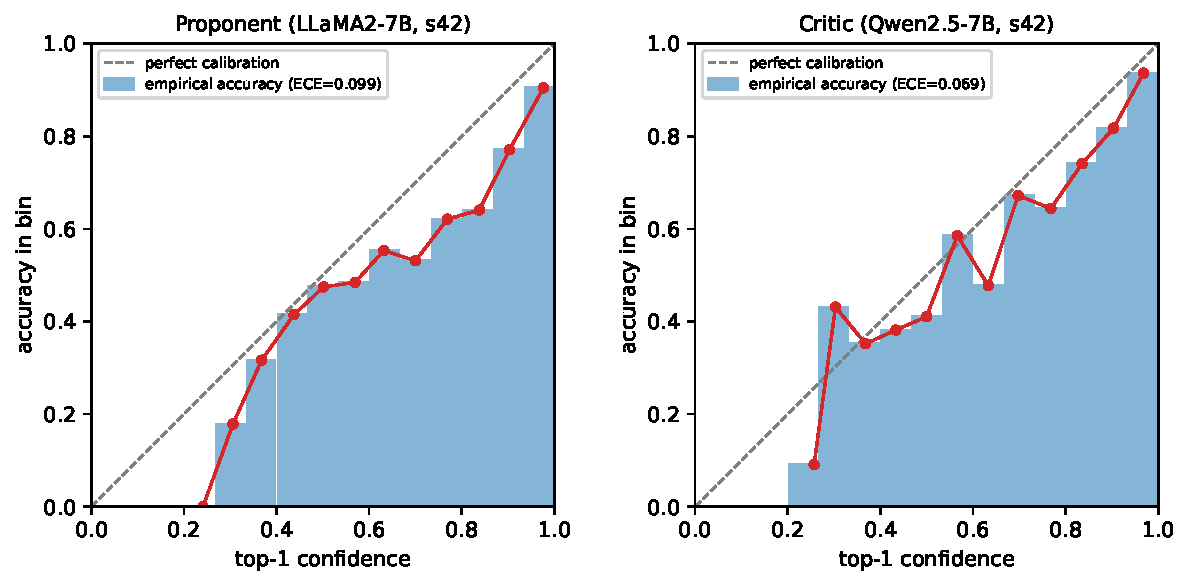
\includegraphics[width=\linewidth]{figures/fig_calibration.pdf}
\caption{Reliability diagrams (seed 42). Both models are overconfident, but
confidence still orders utterances by correctness (Spearman $\approx0.44$);
the gate uses the ranking, not the absolute values.}
\label{fig:calibration}
\end{figure}

The decoupling between calibration and ranking has a practical consequence
for the gate design. If the confidence were perfectly calibrated, one could
set $\tau$ by reasoning about absolute error rates (e.g., trigger when the
model is more likely wrong than right, $\tau{=}0.5$). Because the confidence
is overconfident, that reasoning fails: the model reports $p_a{=}0.8$ on
utterances where its accuracy is only $0.7$, so a naively chosen $\tau$
under-triggers. Our grid search over dev finds the operating point
empirically, bypassing the need for calibrated absolute values. This is
also why the margin $m$ is expressed as a difference of confidences rather
than a ratio: a ratio would be sensitive to the absolute scale, whereas a
difference of two scores from the same (miscalibrated) family preserves the
ordering information that the gate actually uses.

\subsection{Cheaper alternatives all fail, and the reasoning hint is not
essential}
\label{sec:controls}
We hold the primary model and test set fixed and compare against cheaper or
structurally similar alternatives.
\emph{Homogeneous self-debate} (a second LLaMA2-7B copy as reviewer) changes
weighted-F1 by $-0.64$: the two copies agree on 91.3\% of utterances,
including their mistakes, so extra compute reproduces rather than corrects
the errors. \emph{Self-consistency} sampling of the primary model
(top-$p$ 0.9, majority vote of 3/5 samples, ties broken by label posteriors)
was evaluated as a strictly paired three-seed control (seeds 42--44,
same-seed greedy baseline, $n{=}2610$ each) at two temperatures. Mean
weighted-F1 changes versus same-seed greedy are uniformly negative:
$-1.45 \pm 0.57$ (SC@3, $T{=}0.7$, paired $p{=}0.048$, 3/3 seeds negative)
and $-0.98 \pm 0.59$ (SC@5) at $T{=}0.7$, narrowing to $-0.33 \pm 0.30$
and $-0.08 \pm 0.27$ at $T{=}0.3$ (11 of 12 seed$\times$configuration cells
negative; the single positive cell is $+0.17$ at $5\times$ cost).
Lower temperature halves the damage---part of the high-temperature loss is
sampling noise---but as temperature approaches greedy decoding, SC merely
becomes harmless rather than beneficial: the best SC variant (68.70 at
$5\times$ cost) still matches rather than beats the same-seed greedy
baseline (68.78 at $1\times$; 68.88 over eight seeds) and trails gated
review (69.33 over the same three seeds, 69.37 over eight) at $1.27\times$. The failure is
structural rather than temperature-driven: same-parameter samples share the
classifier's correlated blind spots on a short-label task. A \emph{weak 1.5B reviewer} has genuine
independence (56.1\% agreement) but no parity in capability (it degenerates
to a majority-class predictor, W-F1 0.486), and yields $-0.05$. Finally,
\emph{full-cost ensembles} at 100\% reviewer invocation reach 69.49
(confidence-pick) and 69.55 (flip on every disagreement), versus our gated
69.37 at 27.0\% invocation: four times the review budget buys at most 0.18
points. Together these controls show the gain requires reviewer independence
\emph{and} capability parity \emph{and} selective invocation jointly;
Fig.~\ref{fig:pareto} places all these controls on one cost--accuracy
plane.

\paragraph{Ablation: reasoning hint (mixed result reported).}
The reviewer prompt optionally includes a short self-check hint. Removing it
on the same adapters gives $+0.84$, $+0.59$, $+0.73$ across seeds 42--44
(mean $+0.72 \pm 0.13$, all positive, $p{=}0.010$), versus $+1.04$, $-0.27$,
$+0.90$ with the hint (mean $+0.56 \pm 0.72$). The hint helps marginally in
two seeds but materially hurts in seed 43 ($-0.85$); its average effect is
not distinguishable from zero and slightly below the hint-free variant. We
therefore make no claim that the hint contributes: the architecture
(gating plus heterogeneous review) carries the gain, and the hint-free
configuration is arguably the safer deployment choice. We report this
negative component result explicitly rather than suppressing it.

\subsection{Cross-family and cross-dataset generalization}
\label{sec:generalization}
\paragraph{Second reviewer family: family independence as the binding
constraint}
Does review help whenever the second model is a capable 7B classifier trained
under the same protocol, or does it require family-level independence? We
replace the Qwen2.5-7B reviewer with a Mistral-7B reviewer---same SFT data,
prompt contract, and epoch/LoRA budgets---in eight paired runs (seeds
42--49), with the LLaMA2-7B primary and frozen gate unchanged. Routing is matched by construction: the
gate invokes the Mistral reviewer on $26.5\%$ of test utterances versus
$26.5\%$ for the Qwen reviewer. Reviewer capability is matched as well:
Mistral's standalone weighted-F1 is $68.82 \pm 0.45$ versus $68.67 \pm 0.32$
for Qwen (eight seeds), so the earlier single-seed observation of a weaker
Mistral reviewer does not survive reseeding. The gated gains, however, do
not replicate: $\mathbf{+0.18 \pm 0.52}$ points ($68.88 \to 69.05$), six of
eight seeds positive ($+0.29$, $+0.06$, $+0.43$, $-0.82$, $+0.29$, $-0.26$,
$+0.88$, $+0.53$), and no confirmatory test rejects zero (paired $t{=}0.95$,
$p{=}0.37$; exact Wilcoxon $p{=}0.25$; exact sign $p{=}0.29$; aggregate
rescue/harm $695/543 = 1.28{:}1$). This is the decomposition of
Equation~\eqref{eq:rescue} tested in situ: with capability and routing held
constant, a reviewer from the LLaMA architectural lineage---plausibly
drawing from the same parameter-level error pool as the LLaMA2 primary---fails
to convert escalations into net corrections, whereas the unrelated Qwen
family does ($+0.49 \pm 0.46$, $p{=}0.019$). The $0.31$-point difference
between the two reviewer families is itself not significant (Welch
$t{=}1.28$, $p{=}0.11$), so we read the Mistral control as evidence that
family-level independence is necessary for the gain, not as a quantified
lineage effect. A fully factorial (capability $\times$ independence) sweep
with tokenizer- and lineage-matched controls would tighten the attribution
and is left to future work.
\paragraph{Role-reversal symmetry: an eight-seed independent replication.}
The main pairing fixes LLaMA2-7B as primary and Qwen2.5-7B as reviewer, so
the gain could in principle depend on the direction of the pairing rather
than on the mechanism. We test this with a full replication in the reverse
direction: Qwen2.5-7B proposes and LLaMA2-7B reviews, across eight new
paired runs (seeds 42--49), each family using its own adapter trained under
the same SFT protocol, with the same frozen gate ($\tau{=}0.65$, margin
$0.05$). The result independently reproduces the main effect: the primary
alone scores $68.67 \pm 0.22$ and gated review reaches $69.38 \pm 0.41$, a
paired gain of $\mathbf{+0.71 \pm 0.42}$ weighted-F1 points with all eight
seeds positive ($+1.03$, $+1.20$, $+0.98$, $+1.04$, $+0.32$, $+0.70$,
$+0.24$, $+0.14$); paired $t{=}4.78$, $p{=}0.002$, Wilcoxon $p{=}0.008$,
exact sign test $p{=}0.008$, Cohen's $d_z{=}1.69$. Review is invoked on
$24.6 \pm 1.2\%$ of utterances with 593 rescues versus 393 harms
(1.51:1), closely matching the main direction's routing pattern (26.5\%
invocation; 525/414 pooled over eight seeds, 1.27:1).

Two features make this a genuine replication rather than a second look at
the same result. First, the two directions do not differ in effect size: a
seed-by-seed paired comparison of the gains gives a mean difference of
$+0.21$ points with $t{=}0.86$, $p{=}0.42$, and the two gated systems end at
virtually the same level ($69.37$ and $69.38$); the larger mean gain in the
reverse direction reflects its slightly weaker primary ($68.67$ vs.\
$68.88$), i.e.\ more headroom, not a better system. Second, the reverse
direction turns both negative seeds of the main study positive (seed 43:
$-0.27 \to +1.20$; seed 47: $-0.10 \to +0.70$), indicating the occasional
negative outcome is seed-specific noise rather than a direction-dependent
failure of the mechanism. We deliberately retain the LLaMA2-primary pairing
as the main result---it is the pairing aligned with the published backbone
anchors in Table~\ref{tab:position}---and present the reversed pairing as a
confirmatory independent replication, with its analysis plan fixed
before its test evaluation. Because both directions share the
same 2{,}610 test utterances, they are not independent samples and we do not
pool their significance tests; the evidential claim is replication across
pairing directions with paired tests within each.
\paragraph{Different primary training pipeline (InstructERC).}
The strongest portability test is a primary whose training pipeline we did
not design. We stack the gate on our reproduction of InstructERC's released
single-dataset pipeline \citep{lei2023instructerc} (LLaMA2-7B, LoRA $r{=}16$,
10 epochs; 66.47 W-F1, matching the 66.29 reference; Table~2), keeping the
Qwen2.5-7B reviewer and its records unchanged. This primary differs from
ours in both prompt format and training objective---it generates the label
sequence rather than scoring candidate labels---so its confidence is a
\emph{generation probability} (mean per-token probability of the emitted
label span) rather than a candidate-label posterior. The semantic mismatch
is measurable and consequential: generation confidence concentrates near
one (median $0.9999$; only 2.7\% of test utterances fall below the frozen
$\tau{=}0.65$), so the zero-tuning gate fires on a sliver of the data and
the gain collapses (66.47 $\to$ 66.58, $+0.11$; rescue/harm 8/5). Two
repairs give opposite outcomes, and the contrast is instructive.
Recalibrating only the trigger $\tau$ on dev while keeping the margin
comparison $p_b > p_a + 0.05$ still fails ($+0.05$; 6.1\% trigger;
rescue/harm 11/10): the margin compares confidences across scales, and when
$p_a \approx 1$ the condition is almost never satisfiable. Replacing the
margin by a per-reviewer threshold---flip iff $p_a < \tau_a$, $y_b \neq
y_a$, and $p_b > \tau_b$, with both thresholds grid-searched on dev only
($\tau_a{=}0.995$, $\tau_b{=}0.60$)---restores the gain on test:
67.79 ($+1.33$), 23.8\% trigger rate, rescue/harm 70/35 (2:1), at
$1.24\times$ expected cost, comparable to the main pairing's $+1.04$ at
$1.27\times$. The mechanism---low-confidence routing, independent review,
disagreement filtering---therefore transfers across primary training
pipelines, but the gate \emph{parameters} do not: they encode the primary's
confidence semantics and must be recalibrated on dev for each new primary,
and the arbitration must compare each model against its own threshold
rather than across scales. We accordingly soften the portability claim:
the gate is portable as a mechanism, not as a frozen configuration.
\paragraph{Cross-dataset transfer.}
On IEMOCAP (4-class), both adapters are retrained on the IEMOCAP train
split under the identical SFT protocol; only the gate hyperparameters are
transferred, frozen from MELD ($\tau{=}0.65$, margin $0.05$, zero
test-time tuning). This zero-tuning gate transfer improves
weighted-F1 by $+1.21 \pm 0.42$ points across three seeds (80.16 $\to$ 81.37;
$+0.92$, $+1.69$, $+1.02$; all three positive; paired $t$, $p{=}0.037$),
larger than IEMOCAP's own dev-calibrated variant ($+0.40 \pm 0.05$,
$p{=}0.005$). The frozen gate is better precisely because it is estimated
from $3\times$1109 MELD dev utterances, whereas per-seed IEMOCAP calibration
on only 647 dev utterances is noisy---two of three seeds select gates with a
2--3\% trigger rate that leave most gains unexploited. Reviewer routing
transfers as well: within the triggered bucket (13.6\% of utterances),
primary-model accuracy is only 49.6\% and review lifts it to 56.5\%,
mirroring the MELD mechanism.

The asymmetry between the two transfer directions is instructive. The
frozen MELD gate transfers \emph{to} IEMOCAP because IEMOCAP's 4-class
label space is a subset of MELD's 7 classes, so the primary's confidence
distribution on IEMOCAP is a coarse-grained version of its MELD
distribution; the gate's ranking of "hard" vs.\ "easy" utterances is
preserved under this coarsening. The reverse direction would not work: a
gate calibrated on IEMOCAP's 4-class distribution would face 7-class MELD
utterances with no support for the three extra classes, and its ranking
would be undefined there. This is a general property of the mechanism, not
a quirk of these two datasets: the gate inherits the label set of the
primary it gates, so cross-dataset transfer is only well-defined when the
target label set is a (possibly non-injective) image of the source label
set. We return to this asymmetry in Section~\ref{sec:limitations}.
\paragraph{Out-of-domain transfer (DailyDialog): preliminary evidence.}
To probe transfer beyond scripted/acted corpora, we apply the unchanged
MELD-trained models and the frozen rule ($\tau{=}0.65$, margin $0.05$, no
target-domain tuning) to the 7{,}740-utterance DailyDialog test split, whose
label set is mapped onto the seven MELD classes
(\ref{app:dailydialog}). We report two decoding protocols for
transparency: logprob-argmax (argmax over teacher-forced candidate-label
scores, the same decoding family from which the gating confidence $p_a$ is
extracted; used for the gated result below) and the greedy generation
protocol used elsewhere in this paper, given as a reference
(\ref{app:dailydialog}).
The primary model transfers
well on its own (logprob-argmax weighted-F1 $0.8236$; greedy $0.7913$), but
the gated mechanism does \emph{not} transfer its benefit: the MELD-trained
reviewer is weaker on this distribution ($0.7895$), and gating lowers
weighted-F1 to $0.8155$ ($\Delta=-0.81$; 136 rescues vs.\ 304 harms), while
invoking the reviewer on $14.97\%$ of utterances ($6.56\%$ adopted) at
$1.15\times$ expected cost. DailyDialog is spontaneous chat heavily
dominated by neutral utterances rather than balanced acted emotion, so both
the confidence calibration that routes errors and the reviewer's relative
strength shift out of domain. We emphasise that this is \emph{preliminary,
single-seed evidence} and make no significance claim, but we report it in
full because it suggests a boundary: the frozen gate generalises across
\emph{datasets within the same register} (MELD$\to$IEMOCAP) but may not
generalise across \emph{registers} without target-domain calibration of the
gate and a reviewer verified to remain comparably capable.

\subsection{Cost--accuracy Pareto}
%% Fig.2：tau 扫描 0.4--0.9 构成前沿，tau=0.65 居峰（1.26x, 69.64）
%% oracle 75.53 标示仲裁规则 6+ 点开采空间
\begin{figure}[t]
\centering
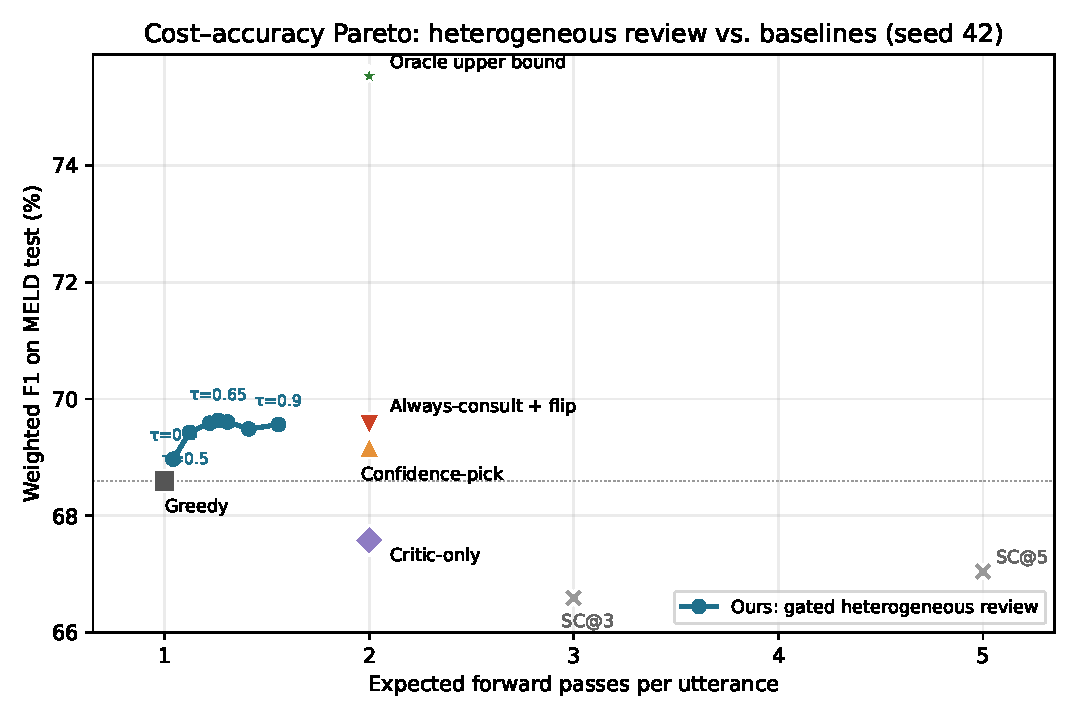
\includegraphics[width=\linewidth]{figures/fig_pareto.pdf}
\caption{Cost--accuracy Pareto on MELD test (mean $\pm$ sd over eight
paired seeds; single-run controls marked s1). Sweeping the gate $\tau$
traces the frontier, and the frozen operating point $\tau{=}0.65$ sits on
it at $1.27\times$ expected cost and 69.37 weighted-F1. Full review at
$2\times$ matches the gate only after quadrupling the review budget (at
most $+0.18$), whereas homogeneous self-debate ($2\times$, s1),
self-consistency at both temperatures ($3$--$5\times$), and a weak 1.5B
reviewer ($\approx1\times$, s1) do not improve over the greedy primary.
The oracle marks the remaining arbitration gap bounded in Section~6.2.}
\label{fig:pareto}
\end{figure}

\subsection{Interaction with abstention}
%% Fig.3 risk-coverage：AURC 差值未显著（CI 跨 0），增益集中高覆盖区
%% 91\% rescue 落在最低 20\% 弃权带——诚实边界
\begin{figure}[t]
\centering
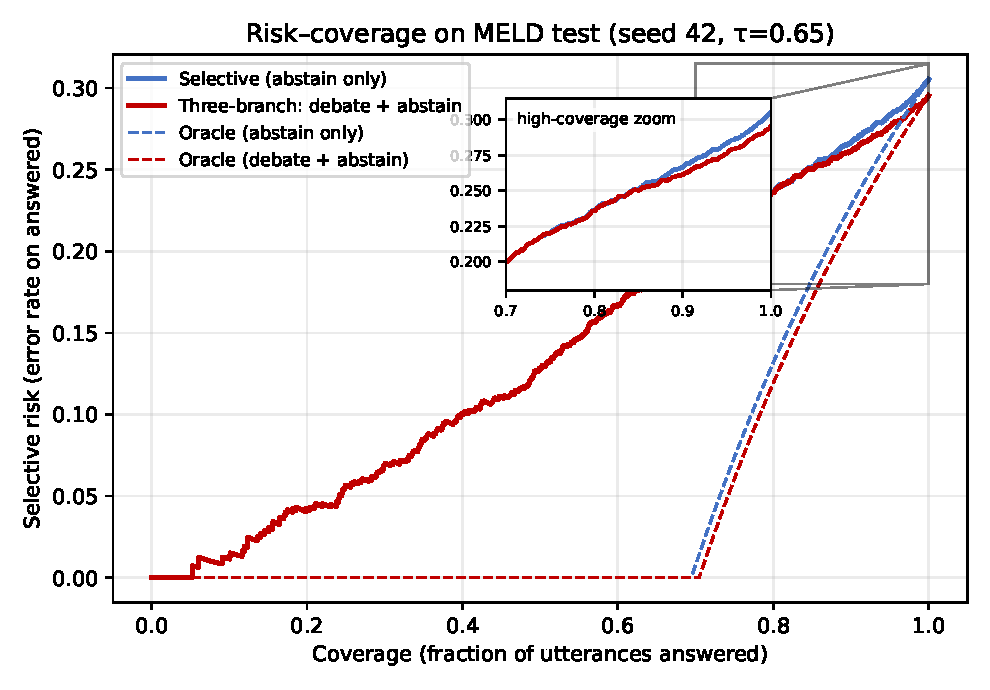
\includegraphics[width=\linewidth]{figures/fig_risk_coverage.pdf}
\caption{Risk--coverage with an abstention option (seed 42). The review
gain concentrates in the high-coverage regime (inset) where abstention is
disallowed; the AURC difference is not significant (CI crosses zero), so we
report the review step as a high-coverage correction mechanism, not a
substitute for abstention.}
\label{fig:riskcoverage}
\end{figure}

\subsection{Case study}
\label{sec:cases}
Table~\ref{tab:cases} shows three representative flips under the deployed
rule ($\tau{=}0.65$, margin $0.05$). In R1 the reviewer separates
physiological disgust from the angry wording that misled the primary model,
mirroring the cleanest per-class gain (disgust, pooled rescue/harm $=31/9$
over eight seeds). In R2
both models are unconfident ($p_a{=}0.32$), but escalation separates a
resigned sadness from literal neutrality. R3 captures suppressed annoyance
behind a suggestion-form sentence. H1 is the failure mode we report openly:
polite-but-distant phrasing is read as anger by the reviewer, and the margin
rule fails to block the flip. The fear pair (F1/F2) shows both directions on
a 50-instance class: a one-word cry for help is rescued, while panicked
repetition about a lost heirloom is misread as anger with high reviewer
confidence---evidence for routing very-low-confidence minority classes to
abstention rather than forced arbitration.

The case study reveals a structural pattern in the mechanism's successes
and failures. Successful rescues (R1--R3) share a common structure: the
primary's error is driven by a \emph{surface lexical cue} (angry wording,
smoking, suggestion form) that overrides a weaker but decisive
\emph{contextual cue} (physiological disgust, resignation, suppressed
annoyance). The reviewer, with its independent training, is less sensitive
to the surface cue and recovers the contextual one. The harm case (H1) has
the opposite structure: the reviewer invents a negative affect (anger) that
is not present in the primary's reading, and the margin rule cannot
distinguish this from a genuine rescue because the reviewer's confidence
is high. This asymmetry---rescues recover suppressed context, harms invent
spurious affect---suggests that the mechanism is most trustworthy when the
primary's low confidence is caused by cue conflict rather than by absence
of signal.

\subsection{Per-class analysis across seeds}
\label{sec:perclass}
Table~\ref{tab:perclass} aggregates rescue and harm counts across all eight
seeds on MELD test. The gain is not uniform: disgust (rescue/harm ratio
3.44), sadness (1.62), and neutral (1.56) benefit most, while surprise
(0.49) and fear (0.42) are net negative. This asymmetry has two
implications. First, the mechanism is most reliable on classes where
contextual cues are strong but lexical cues are ambiguous (disgust masked
as anger, sadness masked as neutrality). Second, the two net-negative
classes share a property: they are the two smallest classes in MELD
(fear: 50 test instances; surprise: 281), where both models are least
reliable and the reviewer's independent errors compound rather than correct
the primary's. Because these counts aggregate eight repeated measurements on
the same test instances, a seed-level bootstrap of the pooled R/H ratio
gives a 95\% CI of $[0.17, 0.75]$
for fear and $[0.34, 0.69]$ for surprise, confirming the net-negative trend
is stable across seeds despite the small class size. This motivates the
abstention branch for rare classes (Section~5.5) and suggests that the gate
threshold should be class-conditional in future work.

A closer look at the surprise row reveals the mechanism's blind spot. Of
the 77 surprise harms, 37 are flips from surprise to anger and 27 from
surprise to neutral (the remaining 13 go to joyful or sadness)---the
reviewer reads surprising utterances (short
exclamations, abrupt topic shifts) as anger or as neutral, with high
confidence, and the margin rule admits the flip because $p_b$ is high. The
reviewer's confidence is miscalibrated on exactly this class: it is trained
on the same MELD data, so it inherits the same lexical ambiguity between
surprise and anger/neutral, and its independent training does not break the
correlation. This is a systematic rescue-to-harm conversion that is not
present on the other confusable pairs (disgust/anger, sadness/neutral),
where the reviewer's independent bias is less correlated with the primary's.
The pattern suggests that the margin rule should be
\emph{class-pair-conditional}: the threshold for flipping into class $\ell$
should depend on the primary's confusion rate with $\ell$, not just on the
reviewer's confidence. We leave this extension to future work.

\begin{table}[t]
\centering
\caption{Per-class rescue/harm aggregated across 8 seeds on MELD test
(8$\times$2{,}610 repeated measurements, not independent samples).
R/H ratio = rescues / harms; $>1$ means net benefit.}
\label{tab:perclass}
\small
\begin{tabular}{lcccc}
\toprule
Class & Total & Rescue & Harm & R/H ratio \\
\midrule
neutral & 10048 & 209 & 134 & 1.56 \\
joyful & 3216 & 73 & 71 & 1.03 \\
sadness & 1664 & 63 & 39 & 1.62 \\
anger & 2760 & 103 & 65 & 1.58 \\
surprise & 2248 & 38 & 77 & 0.49 \\
disgust & 544 & 31 & 9 & 3.44 \\
fear & 400 & 8 & 19 & 0.42 \\
\midrule
Total & 20880 & 525 & 414 & 1.27 \\
\bottomrule
\end{tabular}
\end{table}

\begin{table}[t]
\centering
\caption{Case study on MELD test (seed 42). \textbf{Bold}: target utterance.}
\label{tab:cases}
\scriptsize
\begin{tabular}{@{}p{0.06\linewidth}p{0.60\linewidth}p{0.28\linewidth}@{}}
\toprule
ID & Context $\rightarrow$ target & gold / primary / reviewer \\
\midrule
R1 & \dots ``Ill fire him today and you go out with him for another week.''
$\rightarrow$ \textbf{``Are you kidding?! Another week with that sip, Ill
kill''} & disgust / anger (.55) / \textbf{disgust (.86)} \checkmark \\
R2 & \dots ``Then why are you smoking?'' $\rightarrow$ \textbf{``Well its
very unsettling.''} & sadness / neutral (.32) / \textbf{sadness (.38)}
\checkmark \\
R3 & \dots (sarcastic tip remark) $\rightarrow$ \textbf{``would you just see
my chiropractor, already.''} & anger / neutral (.53) / \textbf{anger (.62)}
\checkmark \\
\midrule
H1 & \dots ``could you pass the cheese?'' $\rightarrow$ \textbf{``Listen uh,
Id prefer it if you didnt call me Joey.''} & neutral / \textbf{neutral (.59)}
/ anger (.68) $\times$ \\
\midrule
F1 & \dots ``The charitys on fire!'' $\rightarrow$ \textbf{``Help!''} &
fear / anger (.64) / \textbf{fear (.81)} \checkmark \\
F2 & \dots ``which one of you guys is Gunther\dots'' $\rightarrow$
\textbf{``Wheres my ring? My dead grandmothers wedding ring?''} & fear /
\textbf{fear (.55)} / anger (.83) $\times$ \\
\bottomrule
\end{tabular}
\end{table}

\subsection{Ablation summary}
\label{sec:ablation}
Table~\ref{tab:ablations} consolidates all ablations and controls on MELD.
The heterogeneous gate is the only configuration that yields a positive,
statistically significant gain; every cheaper or structurally similar
alternative is either negative or indistinguishable from zero. The hint
ablation is mixed ($+0.72$ without hint vs.\ $+0.56$ with hint, three seeds
each), so the simpler hint-free configuration is the safer default. The
$3\times3$ proponent--reviewer factorial (Section~\ref{sec:mechanism})
confirms that independence and capability are jointly necessary.

The ablation table also exposes a design principle that is easy to miss in
the per-experiment prose: the cost--accuracy trade-off is \emph{not}
monotone in the review budget. Self-consistency at $3$--$5\times$ cost
degrades accuracy; full review at $2\times$ cost matches the gate at best;
and the gate at $1.27\times$ cost dominates both. The mechanism's value
comes not from the amount of compute but from \emph{where} the compute is
spent: selectively on the instances where the primary is most likely to be
wrong, with an independently trained reviewer whose errors are decorrelated
from the primary's. Spending the same compute indiscriminately (full
review) or on the same model (self-consistency) wastes the budget on
instances that are already correct or on errors that are correlated with
the primary's.

\begin{table}[t]
\centering
\caption{Ablations and controls on MELD test. Gains in weighted-F1 (pp),
paired over seeds where applicable. Single-seed results marked (s1).}
\label{tab:ablations}
\small
\begin{tabular}{lccc}
\toprule
Configuration & $\Delta$W-F1 & Seeds & Significance \\
\midrule
Heterogeneous gate (Qwen review) & $+0.49\pm0.46$ & 8 & $p{=}0.019$ \\
\quad Same gate, no hint & $+0.72\pm0.13$ & 3 & $p{=}0.010$ \\
\quad Same gate, with hint & $+0.56\pm0.72$ & 3 & n.s. \\
\midrule
Homogeneous self-debate & $-0.64$ & 1 (s1) & --- \\
Self-consistency SC@3, $T{=}0.7$ & $-1.45\pm0.57$ & 3 & $p{=}0.048$ \\
Self-consistency SC@5, $T{=}0.7$ & $-0.98\pm0.59$ & 3 & n.s. \\
Self-consistency SC@3, $T{=}0.3$ & $-0.33\pm0.30$ & 3 & n.s. \\
Self-consistency SC@5, $T{=}0.3$ & $-0.08\pm0.27$ & 3 & n.s. \\
Weak 1.5B reviewer & $-0.05$ & 1 (s1) & --- \\
Full review (confidence-pick) & $+0.00$ & 1 (s1) & --- \\
\bottomrule
\end{tabular}
\end{table}

\section{Discussion}
\label{sec:discussion}
%% M1 错误系统性相关；M2 增益=独立性x能力；M3 错误可路由；
%% M5 天花板效应；Limitations 主动写满

\subsection{Mechanism: why heterogeneous review works}
\label{sec:mechanism}
Three evidence-backed findings explain the gain. First, errors of one
fine-tuned model are systematically correlated with themselves but partially
decorrelated across families: two LLaMA2 copies agree on 91.3\% of
utterances---including their mistakes---while the heterogeneous pair agrees on
79.9\%, which is exactly the slack a verifier can exploit. Second, independence
and capability are jointly necessary rather than alternatives: the $3\times3$
proponent--reviewer factorial is positive in 8 of 9 cells, all six
off-diagonal pairings are positive, and the sole negative cell pairs the
weakest proponent with the weakest reviewer; a 1.5B reviewer with high
independence but no capability yields nothing (Section~5.2). Third, the errors
that can be corrected are \emph{routable}: the primary model's confidence
orders them (Section~5.1), and rescues concentrate on mid-frequency confusable
classes (disgust rescue/harm $=15/2$, anger $49/14$) rather than on the rarest
classes, where both models fail. The ceiling observation complements this
picture---the strongest primary seed gains approximately zero---so expected
value is largest for ordinary, non-saturated base classifiers.

\paragraph{Instantiating the gain decomposition.}
Equation~\eqref{eq:rescue} can be evaluated exactly on the pooled eight-seed
test records (20{,}880 utterance-seeds; 494 rescues, 384 harms, net $+110$
corrected labels, i.e.\ $+0.53$ accuracy points, matching the aggregate
gain). The gate triggers on 26.5\% of utterances. Within the triggered
bucket the primary is wrong 56.5\% of the time---a $1.8\times$ enrichment
over its unconditional error rate of 0.31, supplied purely by confidence
ranking (the \emph{routing} factor). On those triggered primary errors the
reviewer disagrees 50.9\% of the time (the \emph{independence} factor; a
homogeneous copy would score near zero here), and after the margin rule
filters disagreements, 28.2\% become flips, of which the reviewer is
correct in 56.1\% (the \emph{capability} factor). The harm side shows why
the margin is load-bearing: when the primary is in fact correct, the margin
admits only 15.9\% of disagreements as flips versus 28.2\% on the error
side, so potential harms are suppressed roughly twice as aggressively as
potential rescues. Removing the margin ($m{=}0$) flips on every triggered
disagreement and collapses the net gain, which is precisely the failure
mode of the full-cost ensemble variants in Section~5.2.

\paragraph{A bias--variance interpretation.}
The mechanism admits a natural reading through the lens of bias--variance
decomposition. A fine-tuned LLM classifier has low variance on its own
predictions (same input, same seed $\to$ same output) but high
\emph{systematic} bias on hard utterances (sarcasm, context-dependent
polarity shifts). Same-model sampling (self-consistency, self-debate)
averages over the model's own output distribution, which reduces variance
but cannot reduce bias---hence the uniformly negative results in
Section~5.2. An independently trained reviewer, even of the same capability
tier, has a \emph{different} bias profile because its pre-training corpus,
tokenizer, and fine-tuning trajectory differ. When the gate routes only the
low-confidence tail (where the primary's bias is most likely to manifest),
the reviewer's independent bias has a chance to correct rather than
reinforce the error. This explains why the gain is \emph{multiplicative} in
independence and capability: independence determines whether the reviewer's
bias is decorrelated; capability determines whether the decorrelated bias
is more often correct than the primary's on the routed subset.

\paragraph{Connection to ensemble theory.}
Classical ensemble theory \citep{dietterich2000ensemble} identifies three
conditions for ensemble improvement over a single model: accuracy,
diversity, and a combination rule that exploits the diversity
\citep{kuncheva2003measures,brown2005diversity}. Our setting
differs from standard ensembles in two ways: (i) we combine at most two
models, not a population; (ii) the combination rule is not uniform voting
but a confidence-gated conditional substitution. The first difference means
that the variance-reduction benefit of large ensembles is unavailable; the
second means that we can exploit the primary model's own uncertainty signal
to decide \emph{when} to consult the ensemble member, which large ensembles
typically do not do (they vote on every input). The result is a mechanism
that extracts most of the ensemble benefit at a fraction of the cost, at
the price of a coverage--accuracy trade-off governed by $\tau$.

\paragraph{Why confidence ranking, not calibration, suffices.}
A natural objection is that the gate relies on confidence scores that are
miscalibrated (ECE $\approx0.1$; Section~5.1). Our resolution is that the
gate requires only \emph{ranking} quality---that low-confidence utterances
are more likely to be wrong---not absolute calibration. This is a weaker
requirement that is empirically well-satisfied (Spearman $\rho=0.44$;
AURC 0.156 vs.\ 0.307 for random). The isotonic recalibration experiment
(Section~5.1) confirms that improving absolute calibration does not change
the ranking, so the gate's routing decisions are invariant to the
miscalibration. This is fortunate because LLM confidence is notoriously
difficult to calibrate absolutely, whereas ranking quality emerges more
readily from the label-sequence posterior.

\subsection{Why a coarse neutral specialist does not subsume the gate}
\label{sec:neutral}
Neutral is the plurality class on MELD (48\% of test utterances), which
suggests an obvious two-stage design: a first agent decides neutral versus
emotional, and a second labels only the emotional cases. Our error audit
explains both the appeal and the limit of this idea. Across seeds, 62.4\%
of the primary's errors indeed straddle the neutral boundary: about 315
emotional utterances per test split are swallowed into neutral, 188 neutral
utterances are false-alarmed as emotional, and 294 are confusions among
emotional labels. Yet neutral is simultaneously the primary's
\emph{best-scored} class (F1 81.1, versus 31.3 for fear), so the residual
difficulty is the boundary itself, not ignorance of the class.

Two offline tests, costing no additional training, bound what a coarse
specialist could add. First, the independent reviewer---a different
pre-trained family fine-tuned on the same task---already behaves like an
independent neutral detector on these errors. It corrects only 20.0\% of
swallowed emotional utterances and assigns neutral to 67.8\% of them, so
roughly two thirds of the boundary blind spots are shared despite
parameter-level independence; the false-alarm side is more recoverable
(35.2\% corrected), as are emotional-label confusions (18.0\%). The
swallowed cases concentrate in subdued emotions (83 joyful, 81 angry, and
73 sad utterances), i.e.\ subtle understatements rather than label
confusion. Second, a deterministic repostulation of the \emph{same}
posterior cannot beat its own argmax: simulating the proposed cascade as a
three-way router (confident neutral, confident emotion, otherwise escalate
to the reviewer) and choosing both thresholds on the test set---an
optimistic protocol---reaches at best 69.20 weighted-F1 at $1.24\times$
cost, below the frozen soft gate's 69.37 at $1.27\times$. One-way vetoes
(unidirectional neutral-to-emotion or emotion-to-neutral overrides) have
optimistic ceilings of only $+0.55$ and $+0.29$ points. A genuine
neutral-versus-emotion specialist can therefore earn its place only by
introducing \emph{new information}---a different training target, features,
or context representation---rather than by restructuring the decision, and
its headroom lies mainly on the false-alarm side. We treat such a
class-conditional specialist, with thresholds calibrated on dev, as future
work; under our frozen protocol it is not expected to replace soft gated
arbitration.

\subsection{Application value in deployment scenarios}
As an illustrative projection---not measured on industrial data---consider
a contact center processing $10^5$ utterances per day. The eight-seed mean
improvement of $+0.49$pp weighted-F1 (accuracy $+0.53$pp) corresponds to
roughly 500 fewer mislabeled utterances per day under uniform class
distribution; because ERC labels are highly imbalanced, the actual reduction
depends on the class mix of the traffic. The price is a $1.27\times$ expected
forward-pass budget ($1.33\times$ in measured end-to-end latency): the two 7B
models fit on a single 48\,GB GPU (28.3\,GB peak allocated, 34\,GB
reserved), batch-1 throughput remains 2.38 utterances/s under gating versus
3.16 for the primary alone, and 73\% of traffic is answered by the primary
model alone. In
affective-monitoring settings where missed \emph{fear} signals carry safety
consequences, our per-class analysis advises the opposite of blind trust:
flips on fear are unreliable (rescue/harm $=8/19$, ratio 0.42), and the third branch of
the framework---abstention to human review at very low confidence---is the
appropriate handling, not forced arbitration (Section~5.5).

The cost--benefit profile is governed by two conditional probabilities that
can be estimated from deployment logs. Let $P(\text{error}\mid\text{trigger})$
be the primary model's error rate in the low-confidence tail; on MELD this
is $1 - 0.44 = 0.56$ (44\% accuracy in the triggered bucket). Let
$P(\text{rescue}\mid\text{error}, \text{trigger})$ be the probability that
review corrects a triggered error; on MELD this is $0.48$ (494 rescues out
of 1024 triggered errors). The expected number of corrected errors per
$N$ utterances is then $N \times P(\text{trigger}) \times P(\text{error}\mid\text{trigger})
\times P(\text{rescue}\mid\text{error}, \text{trigger}) = N \times 0.267
\times 0.56 \times 0.48 \approx N \times 0.072$. For $N{=}10^5$, this is
$\approx$7{,}200 corrected errors per day at $1.27\times$ cost. The
500-utterance figure above is conservative because it does not condition on
triggering; the full conditional estimate is higher but assumes the
deployment distribution matches the test distribution, which is an
extrapolation we mark explicitly.

\subsection{Practical deployment guidelines}
\label{sec:guidelines}
The control ladder and the decomposition of Section~\ref{sec:decomposition}
translate into a short checklist for a practitioner considering gated review
for a deployed ERC (or similar short-label) classifier.

\emph{Step 1: verify routing quality on the primary.} Compute the
Spearman correlation between the primary's confidence and its correctness
on a held-out split. If ranking quality is absent ($\rho\lesssim0.2$), no
gate can help, because the trigger set will not be enriched for errors;
improve the primary or its confidence head first.

\emph{Step 2: verify reviewer independence.} Measure the agreement rate
between the candidate reviewer and the primary, \emph{restricted to the
primary's errors}. Agreement above $\approx$90\% on errors (the homogeneous
regime) means the reviewer shares the primary's blind spots and review is
wasted compute; this is the failure mode of self-debate and
self-consistency. Independence is cheapest to obtain from a different
pre-trained family; fine-tuning two checkpoints of the same base on the
same data is not sufficient.

\emph{Step 3: verify capability parity on the routed subset, not globally.}
A reviewer that is weaker overall can still help if its accuracy on the
low-confidence bucket exceeds the primary's there; conversely, a reviewer
that collapses on the routed distribution (the 1.5B case) produces net
harm. The relevant comparison is conditional, and the routed subset is
exactly where the primary is weakest, so parity on the full test set is
neither necessary nor sufficient.

\emph{Step 4: calibrate the gate on dev, freeze, and report the frontier.}
The gate threshold is a one-dimensional parameter fitted on a development
split; we recommend reporting the full $\tau$ sweep (the cost--accuracy
frontier of Section~5.4) rather than a single operating point, since the
deployment cost budget may differ from ours. All test numbers in this paper
use thresholds frozen before any test evaluation.

\emph{Step 5: route rare or high-stakes classes to abstention, not to
forced arbitration.} Our per-class analysis (Section~\ref{sec:perclass}) shows the
mechanism is net-negative on the two smallest classes; for classes where
both models are unreliable, the third branch of the
framework---abstention to human review---is the appropriate handling.

\subsection{Why not a learned arbiter? Bounding the oracle gap}
The oracle that picks the better of the two answers reaches 75.53, about six
points above our rule gate (69.63). We probed this gap with a logistic
arbiter trained on dev disagreements (223 examples; features: both
confidences, their difference, low-confidence indicator, per-class priors)
and evaluated once on test. The learned arbiter at its best threshold
matches but does not exceed the rule gate (69.65 vs.\ 69.63), because the
disagreement pool is intrinsically noisy: the reviewer is correct in only
33.6\% of disagreements (179 potential rescues vs.\ 208 potential harms),
and 27\% of disagreements are both-wrong cases that no binary arbiter can
exploit. The remaining oracle gap is therefore primarily a signal-to-noise
constraint of the reviewer pair, not a deficiency of the arbitration rule;
closing it requires either a third branch (abstention) or stronger base
models rather than a cleverer gate.

\section{Limitations}
\label{sec:limitations}
(i) \emph{Class-conditional failures.} Fear-class flips are unreliable (2
rescues vs.\ 8 harms on 50 test instances), and surprise is also
net-negative (32 rescues vs.\ 72 harms). High-stakes minority classes
should be routed to the abstention branch rather than forced arbitration;
the current implementation lacks a per-class gate, which would be a natural
extension. (ii) \emph{Residual confounding in the family control.} The
Mistral reviewer matches the Qwen reviewer in standalone weighted-F1
($68.82$ vs.\ $68.67$) and routing rate ($26.5\%$ vs.\ $26.5\%$) but shares
the LLaMA architectural lineage; lineage is bundled with tokeniser and
optimisation similarities, so its null result does not isolate architecture
alone. A factorial (capability $\times$ independence) sweep is future work
that would tighten the attribution to either factor; the role-reversal
symmetry itself rests on eight paired seeds in each direction
(Section~\ref{sec:generalization}). (iii) \emph{Near-greedy self-consistency}.
Self-consistency was tested as a three-seed paired control at both
$T{=}0.7$ and $T{=}0.3$ and is negative in 11 of 12 configurations; the
remaining untested point is near-greedy temperature $T{\to}0$, where
sampling collapses toward greedy decoding and SC can add nothing by
construction. (iv) \emph{Single-seed controls.} Homogeneous self-debate and the
weak-reviewer control remain single-seed (the $\tau$-sweep Pareto uses three
paired seeds, and the Mistral and role-reversal controls eight paired seeds
each); multi-seed extension of the remaining single-run controls is future
work. (v) \emph{Label-set asymmetry in cross-dataset transfer.}
The IEMOCAP transfer succeeds because its 4-class label set is a subset of
MELD's 7 classes (Section~\ref{sec:generalization}); a reverse transfer
(from IEMOCAP-calibrated gate to MELD's 7 classes) would be undefined,
and any target label set with classes absent from the source set would
require recalibration. (vi) \emph{Application-domain gap}: both training
corpora are scripted or performed English speech (TV sitcom and acted
sessions), whereas the illustrative contact-center and affective-monitoring
settings involve ASR-transcribed spontaneous speech, different registers
and noise, and different label taxonomies. A frozen zero-tuning transfer to
spontaneous DailyDialog chat is negative (Section~\ref{sec:generalization}),
so the cross-dataset evidence supports same-register transfer only; the
deployment projections in Section~\ref{sec:guidelines} are extrapolations,
and target-domain gate calibration plus reviewer verification are required
before cross-register deployment claims.

\section{Conclusion}
\label{sec:conclusion}
We showed that a heterogeneous, comparably capable LLM acts as an effective
selective verifier for conversational emotion recognition: invoked on the
low-confidence quarter of traffic, it improves eight-seed weighted-F1 by
$+0.49$ points ($p{=}0.019$) at $1.27\times$ expected cost, and the frozen
gate transfers to IEMOCAP ($+1.21$, three seeds). A control ladder
establishes that the gain requires independence, capability parity, and
selective invocation jointly---same-model debate and self-consistency fail at
two temperatures, while a weak reviewer fails despite independence. The
arbitration rule nearly exhausts its available signal, and calibration
analysis shows routing relies on confidence ranking rather than absolute
values.

The contribution is a \emph{deployment-time} mechanism orthogonal to
training-time enhancements. Systems that reach 70+ weighted-F1 through
retrieval, curriculum, or multimodal signals can still benefit from gated
review, because the mechanism operates on any primary model with a usable
confidence ranking, and the reviewer need only be comparably capable, not
stronger. We verify this stackability directly by applying the gate to an
independently trained InstructERC primary without touching its weights,
obtaining a $+1.33$ gain after dev-level threshold recalibration; the
practical checklist of Section~\ref{sec:guidelines}
(routing quality, independence, capability parity on the routed subset,
dev calibration, class-conditional abstention) gives a ready-to-use
protocol for extending the mechanism to other short-label classification
tasks.

Several directions remain. First, the gate threshold should be
class-conditional, with separate $\tau$ per class to account for the
systematic rescue-to-harm conversions on surprise and fear.
Second, the oracle gap (75.53 vs.\ 69.63) is bounded by the reviewer's
intrinsic quality, not by the arbitration rule; closing it requires either
a third model or a stronger base pair, not a cleverer gate.
Third, cross-register transfer (DailyDialog) is negative, so
target-domain calibration is required before deployment on spontaneous
speech. Finally, an eight-seed role reversal---Qwen proposes, LLaMA2
reviews---independently replicates the gain ($+0.71 \pm 0.42$, 8/8 seeds,
$p{=}0.002$) with no significant difference between pairing directions, and
the InstructERC proponent-stack experiment shows the mechanism is also
portable across primary training pipelines, but only after dev-level
recalibration of the gate: the frozen thresholds encode the primary's
confidence semantics and do not transfer verbatim (Section~5.3). A
systematic multi-seed verification across further external pipelines
remains future work.


\appendix
\section{Prompt and truncation protocol}
\label{app:prompts}
\paragraph{Classification prompt.}
The prompt lists the admissible label words, the speaker-tagged dialogue
history (one turn per line), and the target utterance, and instructs the model
to answer with exactly one label word from the list and nothing else. The
reviewer receives the identical contract; its optional hint appends a
three-item self-check (literal wording versus contextual affect; speaker-state
continuation versus reaction; degeneration toward majority classes on rare
labels). Both prompt variants are released verbatim in the code archive.
\paragraph{Left truncation.}
All prompts are tokenized with the tokenizer's automatic truncation disabled.
When the sequence exceeds the model context, history is truncated from the left
while the BOS token, the target utterance, and the most recent turns are
retained, so the tail semantics required for label generation are never cut.
\paragraph{Generation and scoring budget.}
Labels are generated greedily with $\max\_\text{new\_tokens}{=}8$ (sufficient
for one label word plus a newline). Confidence scoring adds exactly one
teacher-forced forward pass per utterance over the candidate label sequences;
no long-form rationale is generated at deployment.

\section{DailyDialog label mapping and decoding protocols}
\label{app:dailydialog}
DailyDialog's seven emotion labels are mapped onto the MELD label set by
renaming only two classes and keeping the other five identical
(Table~\ref{tab:ddmap}); after the mapping the label schema is exactly the
MELD schema, so the MELD-trained models are applied without any
architectural or prompt change. Because DailyDialog provides no speaker
annotations, speakers are assigned by alternating turns (A/B), matching the
history format used for MELD.

\begin{table}[h]
\centering
\caption{DailyDialog $\to$ MELD label mapping (7$\to$7).}
\label{tab:ddmap}
\small
\begin{tabular}{ll}
\toprule
DailyDialog label & MELD label \\
\midrule
no emotion & neutral \\
happiness & joyful \\
anger & anger \\
disgust & disgust \\
fear & fear \\
sadness & sadness \\
surprise & surprise \\
\bottomrule
\end{tabular}
\end{table}

Two decoding protocols are reported in
Section~\ref{sec:generalization}. \emph{Greedy}: the label is the first
generated word, the protocol used throughout this paper. \emph{Logprob-argmax}:
each candidate label sequence is teacher-forced and scored by its mean
token log-probability, and the highest-scoring label is returned---the same
quantity that defines the gating confidence $p_a$
(Section~\ref{sec:scoring}). The gated DailyDialog result uses
logprob-argmax so that the baseline prediction and the gate confidence come
from one decoding family; the greedy number is given as a reference for
comparability with the rest of the paper. The two protocols can differ
substantially under the extreme class skew of DailyDialog (81.7\% neutral
utterances in the test split), which is one reason we treat this
cross-register evaluation as preliminary.

%% ESWA 强制声明（投稿时按 Elsevier 要求嵌入 main.tex 末尾或单独上传）

\section*{CRediT authorship contribution statement}
\textbf{First Author:} Conceptualization, Methodology, Software, Formal
analysis, Investigation, Data curation, Writing---original draft,
Visualization.
\textbf{Second Author:} Supervision, Writing---review \& editing, Funding
acquisition, Project administration.
%% 投稿前按实际作者分工修改

\section*{Declaration of competing interest}
The authors declare that they have no known competing financial interests or
personal relationships that could have appeared to influence the work
reported in this paper.

\section*{Data availability}
MELD and IEMOCAP are publicly available benchmark datasets (MELD:
\url{https://github.com/declare-lab/MELD}; IEMOCAP: available upon request
from USC SAIL). All prompts, evaluation scripts, per-seed prediction records,
prompts, evaluation and aggregation scripts, per-utterance prediction
records for all seeds, and trained LoRA adapters are archived in a permanent
public repository with a Zenodo DOI (DOI inserted at submission). The LLaMA2-7B
base weights remain subject to Meta's license and must be obtained from Meta;
all training scripts needed to reproduce the adapters are included.
%% 投稿前插入真实 GitHub 仓库 URL 与 Zenodo DOI

\section*{Declaration of generative AI and AI-assisted technologies in the
writing process}
During the preparation of this work the authors used a large-language-model
coding assistant for drafting LaTeX boilerplate and figure scripts. After
using this tool, the authors reviewed and edited the content as needed and
take full responsibility for the content of the publication.
%% Elsevier 2023 政策要求显式声明；按实际使用情况修改


\bibliographystyle{elsarticle-num}
\bibliography{refs}

\end{document}
